\documentclass[12pt]{article}

\usepackage{a4wide}
\usepackage{amssymb}
\usepackage{framed}
\usepackage{graphicx}
\setlength{\parindent}{0pt}

\title{Fun with Solvers \\ \large -- A manual for the riddles --}
\author{Wilhelm Simus}

\begin{document}
	\maketitle
	\thispagestyle{empty}
	\newpage
	
	\section*{Sudoku}
	
	\subsection*{The Rules}
	
	\begin{minipage}[t]{0.55\linewidth}
		\strut\vspace*{-\baselineskip}\newline		
		The classic Sudoku game - as depicted on the left - involves a grid of 81 squares. The grid is divided into nine blocks, each containing nine squares.\\
		
		The rules of the game are simple: each of the nine blocks has to contain all the numbers 1-9 within its squares. Each number can only appear once in a row, column or box.
	\end{minipage}
	\hspace*{0.1\linewidth}
	\begin{minipage}[t]{0.35\linewidth}
		\strut\vspace*{-\baselineskip}\newline 
		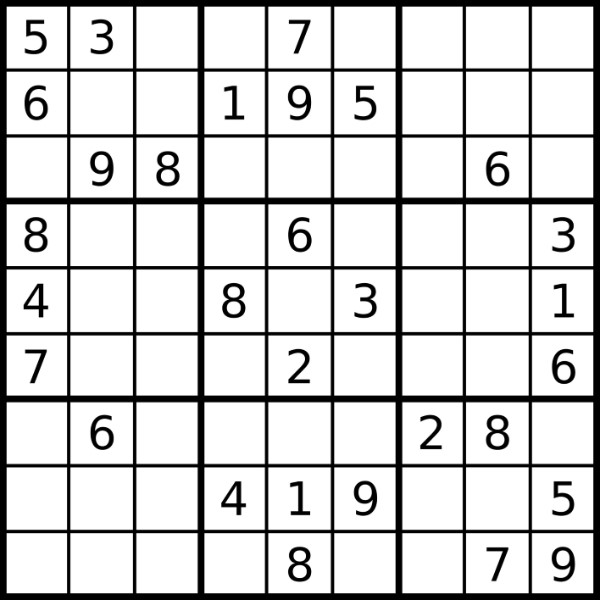
\includegraphics[width = \linewidth]{img/sudoku.jpg}
	\end{minipage}
	
	\subsection*{Example}
	
	As an example we look at a Sudoku riddle in which everything is already solved, except one of the nine blocks.
	%TODO: Insert Sudoku example
	
	\subsection*{Clues}
	
	In this section we collect different clues to look for when solving a Sudoku riddle. These clues can either be used for solving a given riddle manually or be implemented into a solver (which I will do in this project).
	
	\newpage
	
	\section*{Kakuro}
	
	\subsection*{The Rules}
	
	*insert rules here*
	
	\subsection*{Example}
	
	*insert example here*
	
	\newpage
	
	\section*{Shikaku}
	
	\subsection*{The Rules}
	
	*insert rules here*
	
	\subsection*{Example}
	
	*insert example here*
	
	\newpage
	
	\section*{SumSum}
	
	\subsection*{The Rules}
	
	*insert rules here*
	
	\subsection*{Example}
	
	*insert example here*
	
	\newpage
	
	\section*{Picross}
	
	\subsection*{The Rules}
	
	*insert rules here*
	
	\subsection*{Example}
	
	*insert example here*
		
\end{document}